\section{Motivation}
\label{sec:motivation}

\subsection{Channel Model}
\label{sec:model}

\begin{enumerate}
	\item The Assumed Channel Model
	\begin{enumerate}
		\item WiFi networks operate at high SNR.
		\item Most packet errors are due to interference from other users.
	\end{enumerate}

	\item Interference between two users
	\begin{enumerate}
		\item Either user A or user B starts to transmit first, etc...
	\end{enumerate}

\subsection{Sending Incremental Redundancy}
\label{sec:ir}

	\item A System of linear equations
	\begin{enumerate}	
		\item Decoding involves solving for n-unknowns and this is possible when the access point receives at least n-independent equations
		\item <Insert Analysis of necessary number of equations needed for successful decode>
	\end{enumerate}

	\item Ways to Send Incremental Redundancy
	\begin{enumerate}	
		\item How much to send? (Zigzag sends $\beta=1$)
		\item The degree to send? (Zigzag uses degree 1)
	\end{enumerate}

\subsection{Code Structure}
\label{sec:structure}

	\item Random Codes
	\begin{enumerate}	
		\item These types of codes are known to do well for i.i.d. noise channels.
		\item In order to get benefits of randomness, it is necessary to increase the degree to a moderately high value.
		\item In addition, increasing the degree also increases the encoding/decoding complexity.
	\end{enumerate}

	\begin{figure}[t]
	\centering
	\vspace*{-0.1in}
	\subfigure[Performance of Random Code vs. Degree d] {
	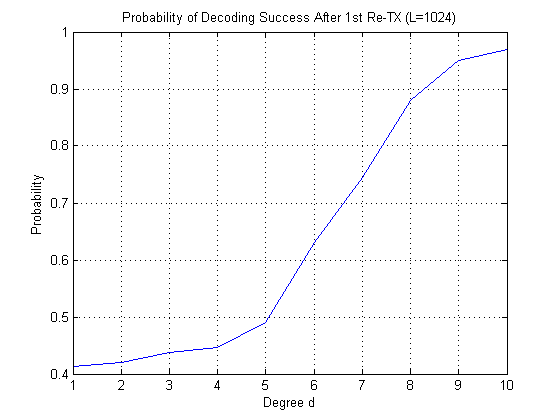
\includegraphics[width=.9\columnwidth]{./figs/prob_rndCode_deg_1to10.png}
	\label{fig:random_vs_d}
	}
	\vskip -0.5em
	\caption{Probability of Success on First Re-Transmission (Random Code) ($\beta=0.75$)}
	%\vskip -1em
	\end{figure}

	\item Structured Codes
	\begin{enumerate}	
		\item Is there some way to get performance close to that of random codes with less complexity?
	\end{enumerate}

	\begin{figure}[t]
	\centering
	\vspace*{-0.1in}
	\subfigure[Comparison of Fold Performance vs. Random] {
	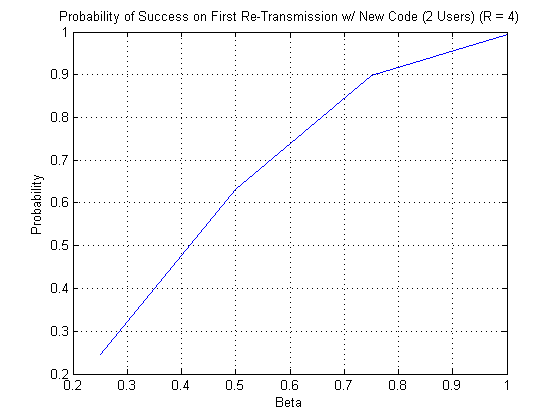
\includegraphics[width=.9\columnwidth]{./figs/prob_newCode_success_2users_b25to100.png}
	\label{fig:fold_2user}
	}
	\vskip -0.5em
	\caption{Probability of Success on First Re-Transmission (Folding)}
	%\vskip -1em
	\end{figure}


\begin{enumerate}
	\item How is Folding Applied (Degree 2)?
	\begin{enumerate}
		\item The code has one parameter $\beta$, $0\leq\beta\leq1$, which controls the amount of incremental redundancy.
		\item For a length N packet, the original bits are given by samples $x_1,x_2,...,x_N$ while the code bits are given by $c_1,c_2,...,c_N$.
		\item For a parameter $\beta$, the length of the codeword becomes $int(\beta n)$.
		\item $\beta\leq 0.5$
		\begin{enumerate}
			\item  $c_i=x_{i} + x_{N-i}$
		\end{enumerate}
		\item $\beta>0.5$
		\begin{enumerate}
			\item  $c_i=x_{i} + x_{i+\frac{N}{2}}$
		\end{enumerate}
	\end{enumerate}

	\item How does this work with 3 or more users?
	\begin{enumerate}
		\item Folding using degree 2 performs similarly to random codes of degree $4\sim6$.
	\end{enumerate}

	\begin{figure}[t]
	\centering
	\vspace*{-0.1in}
	\subfigure[Comparison of Fold Performance vs. Random] {
	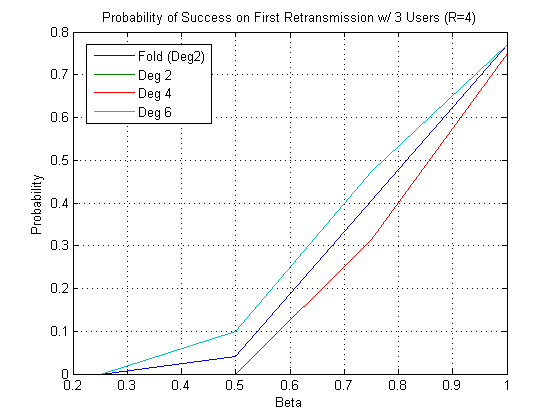
\includegraphics[width=.9\columnwidth]{./figs/prob_rndCode_b25to100_deg2to6_R4_3users.png}
	\label{fig:fold_2user}
	}
	\vskip -0.5em
	\caption{Probability of Success on First Re-Transmission}
	%\vskip -1em
	\end{figure}

 \end{enumerate}
\end{enumerate}




%%	\item How is Folding Applied for (Degree n)?
%%	\begin{enumerate}
%%		\item Maximum Distance between any 2 data symbols is defined as: $D_{m}\doteq int(\frac{N}{n})$.
%%		\item Step size s, $s\doteq mod(i-1,D_m)$.
%%		\item Increment size t, $t\doteq mod(int(\frac{i}{D_m}),n)$
%%		\item ($s \leq \frac{D_m}{2}$)
%%		\begin{enumerate}
%%			\item $c_i=\sum_{k=0}^{n-1}x_{1+s+(D_m-t)k}$
%%		\end{enumerate}
%%		\item ($s > \frac{D_m}{2}$)
%%		\begin{enumerate}
%%			\item $c_i=\sum_{k=0}^{n-1}x_{N-s+(D_m-t)k}$
%%		\end{enumerate}